\section{Numerical examples}

In this section, the proposed coupled mechanical-micromorphic damage HHO method is evaluated on
classical test cases taken from the literature.
The reader can refer to XXX regarding technical aspects. 
The notation
HHO($k,l$) relates to the HHO element of order $k$ on faces, and order $l$ in the
cell.

The tests presented in this section have been performed using an
\texttt{python} implementation freely available on github: \url{https://github.com/davidsiedel/h2o_paper}.

% ---------------------------------------------------------
% PARAGRAPH
% ---------------------------------------------------------
\paragraph{Stabilization parameter}

To ensure coercivity of the HHO method, the so-called \textit{stabilization} parameters
$\DisplacementStabilizationFactor$ and $\MicromorphicDamageStabilizationFactor$, that relate to the stiffness of the elastic interface introduced in Section \ref{sec_hdg_element_equilibrium}, needs be chosen according to the material under study. In \cite{di_pietro_hybrid_2015}, a value of
order $2 \mu$ is advocated for the displacement problem, where $\mu$ denotes the shear modulus of the
material. This value is used for all test cases in the present section. Similarly the micromorphic damage stabilization parameter $\MicromorphicDamageStabilizationFactor$
is chosen in agreement with the stiffness of the micromorphic damage problem, and is equal to $G_c$.

\subsection{Uniaxial rod}
\label{sec_uniaxial_rod}

\paragraph{Specimen and loading}

This benchmark is a tensile test on a uniform rod, with an imperfection at the center.
The rod has an length $L = 1$ mm and a width $l = 0.1$ mm.
A vertical displacement $u$ is imposed at the top of the rod.
The simulation is performed until the limit load corresponding to an internal displacement of $0.2$ mm is reached.

% ---------------------------------------------------------
% PARAGRAPH
% ---------------------------------------------------------
\paragraph{Material behaviour}

The mechanical potential involves a degradation function $g(d)$ acting on the spherical part of the elastic energy of the material such that
%
%
%
\begin{equation}
    \psi_{\tensoriis{F}, \DamageField} (\TransformationGradientField, \DamageField) = g(\DamageField) \, \psi_{sph}(\TransformationGradientField) + \psi_{dev}(\TransformationGradientField)
\end{equation}
%
%
%
where $g(d) = (1 - d)^2$ in order to recover the AT2 model \cite{bourdin_numerical_2000}.
The potentials $\psi_{sph}$ and $\psi_{sph}$ are based on a devatoric-spherical split of the
Hooke tensor for a linear elastic material.
%
%
%
The micromorphic damage and damage potentials are chosen such that
%
%
%
\begin{subequations}
    \label{eq_micromorphic_rod_damage_potentials}
    \begin{alignat}{1}
        \psi_{\DamageField, \MicromorphicDamageField} (\DamageField, \MicromorphicDamageField)
        &
        =
        \frac{1}{2} H_{\chi}(\DamageField - \MicromorphicDamageField)^2
        \label{eq_micromorphic_rod_damage_potentials:eq0}
        \\
        \psi_{\DamageField} (\DamageField)
        &
        =
        \frac{G_c}{2 \ell_c} \DamageField^2
        \label{eq_micromorphic_rod_damage_potentials:eq1}
        \\
        \psi_{\MicromorphicDamageGradientField} (\MicromorphicDamageGradientField)
        &
        =
        A_{\chi} \MicromorphicDamageGradientField \cdot \MicromorphicDamageGradientField
        \label{eq_micromorphic_rod_damage_potentials:eq2}
    \end{alignat}
\end{subequations}
Moreover, the small strain hypothesis is assumed for this test case.
%
% 
% 
\begin{figure}[H]
    \centering
    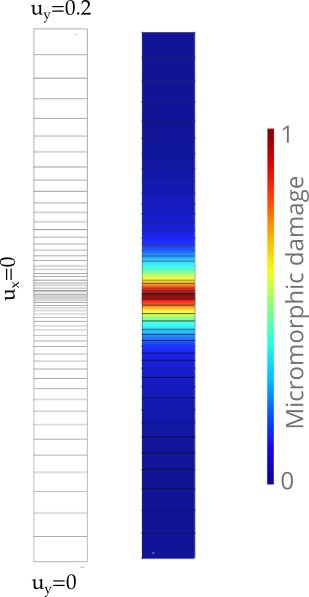
\includegraphics[width=5.cm]{../chapter_004_hho_micromorphic/figures/rod.png}
    \caption{Mesh and micromorphic damage at the last time step}
    \label{fig_rod_micromirphic}
\end{figure}

% ---------------------------------------------------------
% PARAGRAPH
% ---------------------------------------------------------
\paragraph{Displacement along the radius}

The force deflection curve of the experiment is given in Figure \ref{fig_rod_micromirphic_cruve}. The results obtained with the HHO formulation are compared to those provided by
the \texttt{MFEM} library, and are in agreement with those provided by a standard Lagrange discretization.
%
% 
% 
\begin{figure}[H]
    \centering
    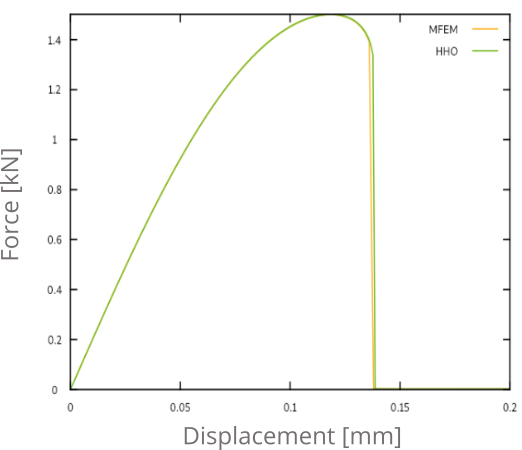
\includegraphics[width=7.cm]{../chapter_004_hho_micromorphic/figures/rod_curve.png}
    \caption{...}
    \label{fig_rod_micromirphic_cruve}
\end{figure}

\subsection{Matrix fiber specimen}

% ---------------------------------------------------------
% PARAGRAPH
% ---------------------------------------------------------
\paragraph{Specimen and loading}

The last application consists of a two dimensional plate that is subjected to uniaxial
extension. The plate (or matrix) is clamped around a fiber of radius $0.2$ mm (representated by the hole in the mesh).
The matrix is a square of length of $1$ mm. A vertical
displacement $u_y = 0.2$ mm is imposed at the top, as shown in Figure \ref{fig_matrix}.

% ---------------------------------------------------------
% PARAGRAPH
% ---------------------------------------------------------
\paragraph{Behaviour law}

The same behavior law as that in \ref{sec_uniaxial_rod} is considered for the present test case.
%
% 
% 
\begin{figure}[H]
    \centering
    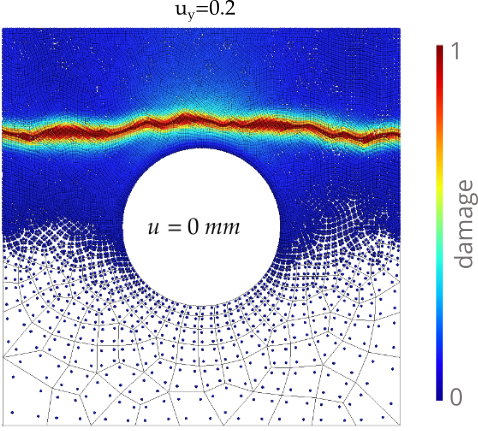
\includegraphics[width=7.cm]{../chapter_004_hho_micromorphic/figures/plate.png}
    \caption{...}
    \label{fig_matrix}
\end{figure}

% ---------------------------------------------------------
% PARAGRAPH
% ---------------------------------------------------------
\paragraph{Load deflection curve}

The load-displacement curve is plotted
in Figure \ref{fig_matrix_curve}, and gives similar results to that obtained with a standard Lagrange discretization.
%
% 
% 
\begin{figure}[H]
    \centering
    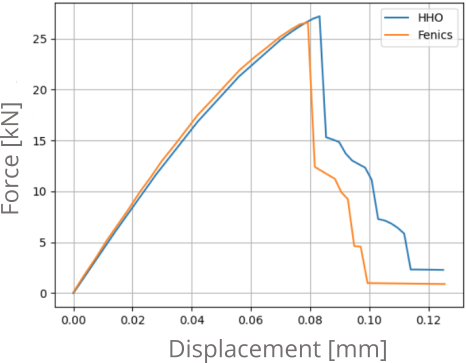
\includegraphics[width=7.cm]{../chapter_004_hho_micromorphic/figures/plate_curve.png}
    \caption{...}
    \label{fig_matrix_curve}
\end{figure}